\documentclass[10pt,letterpaper]{article}
\usepackage[T1]{fontenc}
\usepackage{amssymb}
\usepackage{amsmath}
\usepackage{braket}
\usepackage{enumerate}
\usepackage{graphicx}
\usepackage[margin=0.5in]{geometry}
\usepackage{xcolor}
\title{Introduction to Quantum Electronic Devices and Applications}
\author{Jeremy Chen}
\date{February 9, 2026}
\begin{document}
	\maketitle
	
\begin{enumerate}[\textbf{\arabic{enumi}. }]

\item \textbf{Finite Square Well: Quantum Wells of AlGaAs LEDs}

Quantum wells in LEDs are formed by joining materials with different electronic structures to create a double heterojunction, as shown below. The resulting conduction band offset $\Delta E_{c}$ creates a potential well that can confine electrons.

As discussed in Problem 4 of Homework 2, the infinite square well provides a rough approximation for the energy levels and wave functions inside an LED’s quantum wells. A more realistic model treats the quantum wells as finite square wells instead. The material system shown below is commonly used for generating red and infrared light, where optical transitions occur from the conduction band quantum well to the valence band quantum well,
\begin{figure}[h!]
\centering
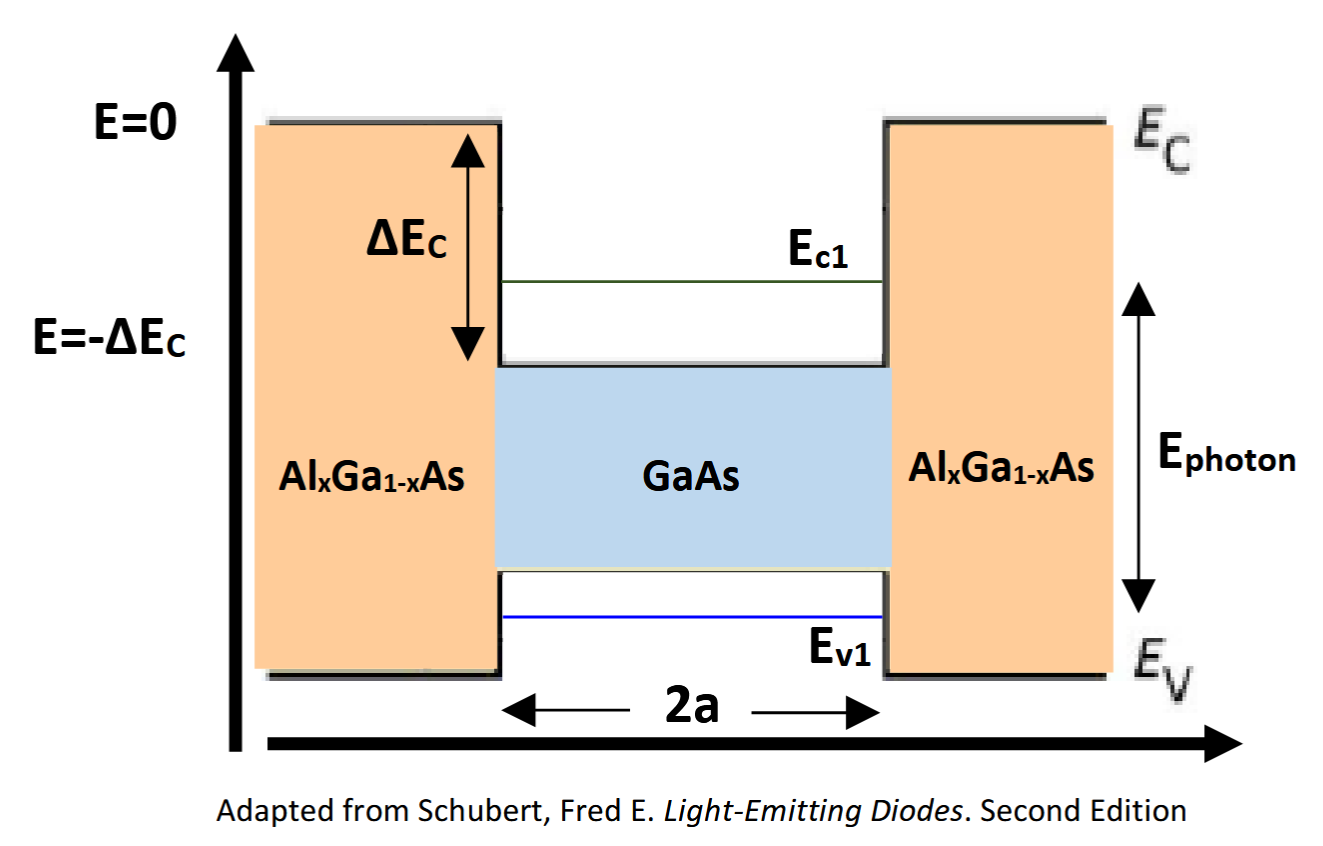
\includegraphics[width=0.4\linewidth]{Screenshot 2026-02-09 192352.png}
\end{figure}

where $\Delta E_{c} = 0.4eV$ is the conduction band offset and the well has a width of $w = 2a = 2nm$. Assume the electrons in the well have an effective mass of $m_{e} = 0.067m_{0}$, where $m_{0}$ is the mass of a free electron.

\begin{enumerate}[a) ]

\item How many bound states does this finite square well support? What are their energies?

\color{violet}
The energies of a finite square well are given by $E_{n} = \frac{n^{2}\pi^{2}\hbar^{2}}{2mL^{2}}$. Here, $a$ is given by $2a = 2nm$. The ground state would have energy
$$E_{0} = \frac{1^{2}\pi^{2}\hbar^{2}}{2m_{0}(2 * 10^{-9})^{2}} = 6.03 * 10^{-20}J = 0.094 eV$$
whereas the first excited state would have energy
$$E_{1} = 0.376 eV$$
Since the conduction band only supports $0.4 eV$ at most, this finite square well only supports 2 bound states. 
\color{black}

\item Sketch the wave functions $\psi_{n}(x)$ for the bound states you found in part a). You do not need to label absolute values of the wave function’s amplitude (i.e. no normalization is necessary).

\item In order to emit a photon, an electron in a bound state of the conduction band quantum well must undergo a downward transition in energy to a bound state of the valence band quantum well. Assuming that the energy between these two states is
$$E_{photon} = 2(E_{c1} + \Delta E_{c}) + E_{g}$$
where $E_{c1}$ is the ground state of the conduction band quantum well and $E_{g} = 1.42 eV$ is the bandgap energy of GaAs, what are the wavelength and color of the emitted photon? 

\color{violet}
The energy of the transition photon is 
$$E_{photon} = 2(0.094 + 0.4) + 1.42 = 2.408 eV = 3.858 * 10^{-19} J$$
The relation between energy and frequency is $E = hf$, so the frequency of the photon is
$$\frac{E_{photon}}{h} = \frac{3.858 * 10^{-19} J}{6.626 * 10^{-34}} = 5.822 * 10^{14} Hz$$
The relation between frequency and the speed of light is $c = \lambda f$, so the wavelength is
$$c = \lambda f = \frac{c}{f} = 5.153 * 10^{-7} m$$
which is around the range of green light. 
\color{black}

\item Accurately controlling the width of a quantum well during the growth process is a major challenge. How do the bound state energies change when the well becomes wider vs. narrower? 

Calculate what the wavelength and corresponding color of the emitted photon if the actual width of the quantum well is 20\% larger than designed (w = 2a → w = 2.4a). Also determine the wavelength and color when the well is 20\% smaller than designed (w = 2a → w = 1.6a).

\color{violet}
Making the well wider decreases the bound state energies, whereas making the well narrower increases the energies. When the well is 20\% wider, the ground state energy is
$$E_{photon} = \frac{1^{2}\pi^{2}\hbar^{2}}{2m_{0}(2.4 * 10^{-9})^{2}} = 0.065 eV$$
which translates to a wavelength of $5.279 * 10^{-7} m$, which is still green. When the well is 20\% narrower, the ground state energy is 
$$E_{photon} = \frac{1^{2}\pi^{2}\hbar^{2}}{2m_{0}(1.6 * 10^{-9})^{2}} = 0.147 eV$$
which has wavelength of $4.936 * 10^{-7} m$, which is cyan. 
\color{black}

\end{enumerate} 

\item \textbf{Gate Current Leakage in MOSFETs}

MOSFETs (metal-oxide-semiconductor field effect transistors) consist of a stacked structure of gate metal, insulating $\text{SiO}_{2}$, and semiconductor. A voltage applied to the gate controls the conductivity of the semiconductor beneath the oxide. When the electric field across the oxide becomes sufficiently large, the energy barrier takes on a thin trapezoidal or triangular shape, allowing electrons to tunnel or “leak” through the gate oxide into the metal, as illustrated on the left. This tunneling current does not contribute to the intended device operation, but wastes power and should be minimized.

Although we cannot solve this problem with the tools available to us so far, we can obtain a lower bound on the tunneling probability and current density by approximating the rectangular oxide as a rectangular barrier, as shown on the right.

\begin{figure}[h!]
	\centering
	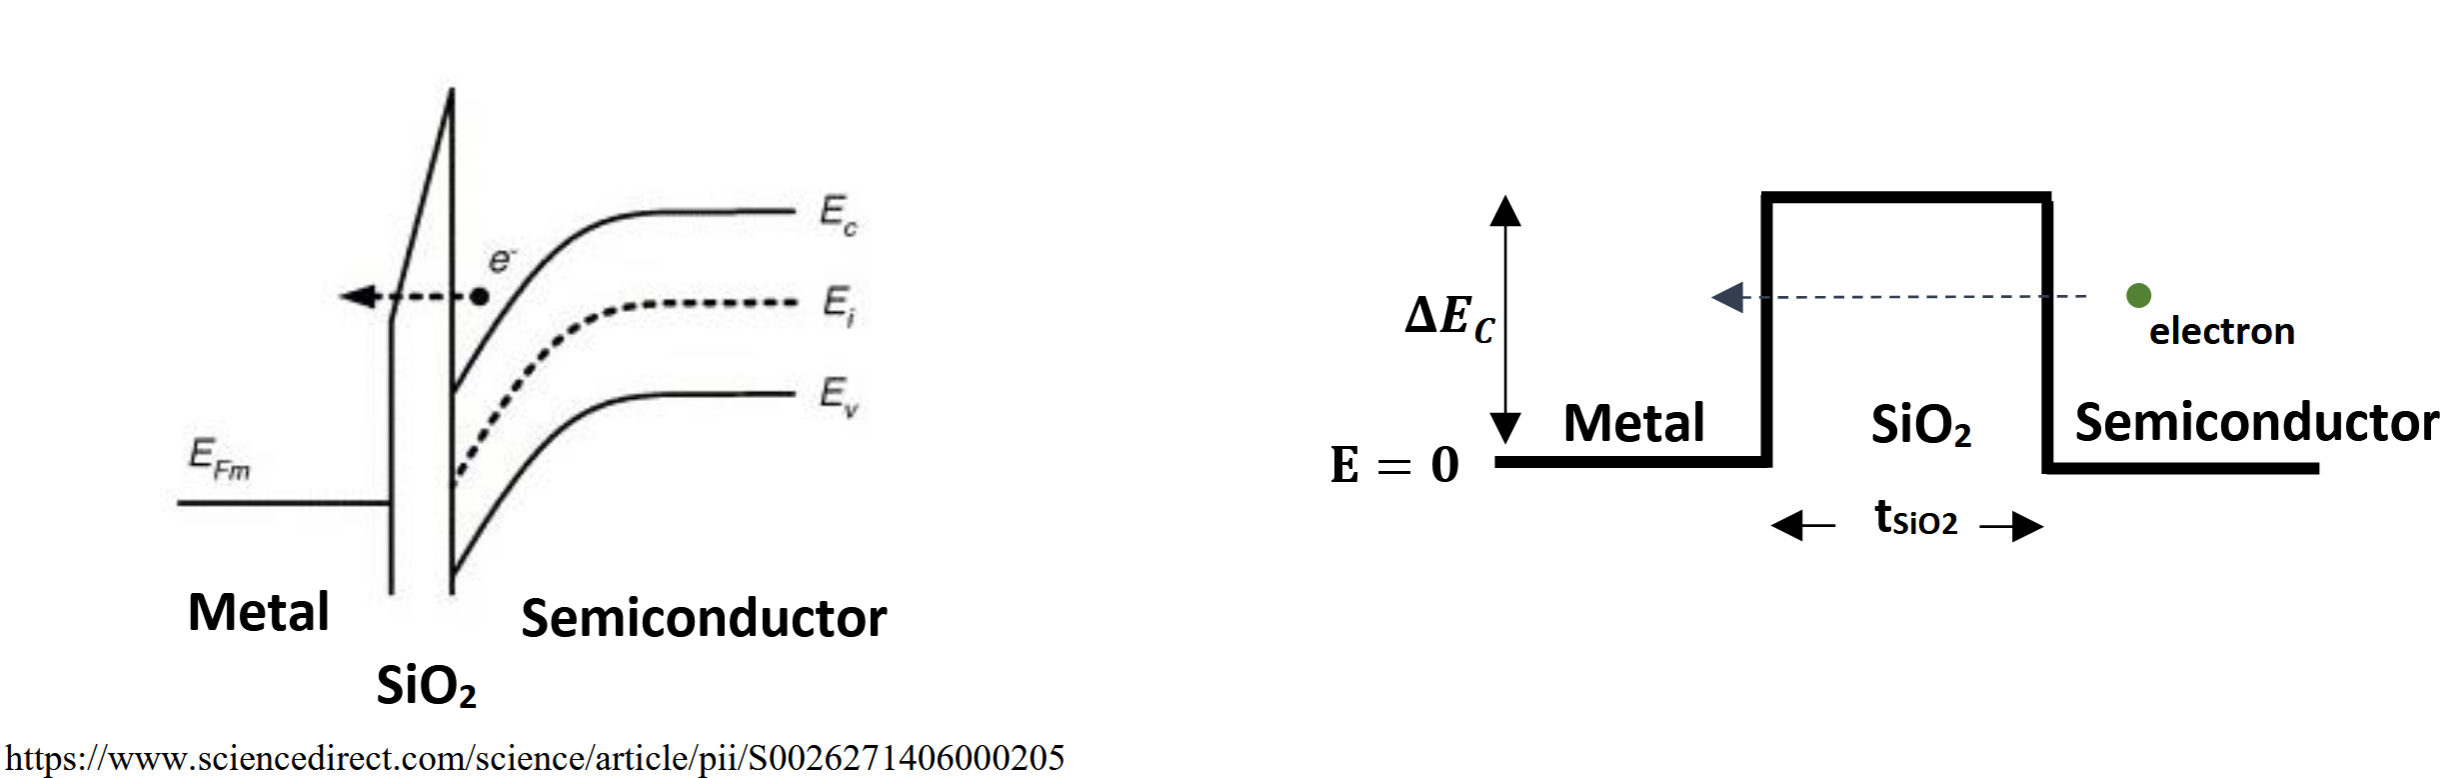
\includegraphics[width=0.9\linewidth]{Screenshot 2026-02-10 182031.png}
\end{figure}

\begin{enumerate}[a)]

\item In the year 1987, gate oxides of the thickness $t_{\text{SiO}_{2}} = 10 nm$ were fabricated. If the oxide barrier height on the semiconductor side is approximately $\Delta E_{c} = 3.2 eV$ and an electron (with mass $m_{0}$) has energy $E = 1.0 eV$, what is the probability that the electron will tunnel from the semiconductor through the oxide and into the metal?

\color{violet}
Given that this is a rectangular barrier, the transmission probability is given by the following equation
$$T = \frac{|t|^{2}}{|1|^{2}} = \frac{1}{1 + \frac{V_{0}^{2}\sinh^{2}(KW)}{4E(V_{0} - E)}}$$
Here, the potential of the system is given by $\Delta E_{c}$, and $k$ is proportional to the given $1.0 eV$. So the reformulated equation would be result in a total transmission probability of 1. 
\color{black}

\item If a current density of magnitude
$$J_{i} = \frac{qnv}{2} = qn\sqrt{\frac{E}{2m_{0}}}$$
is incident on the barrier from the semiconductor side, where $n = 10^{18}\text{cm}^{-3}$ is the electron density and $q$ is the elementary charge, how much of this current density (in $\text{A/cm}^{2}$) is transmitted from the semiconductor into the metal?

\color{violet}
The amount of current transmitted to the other side will remain constant, so the the density would be calculated as
$$J_{o} = 1.602 * 10^{-19} * 10^{18} \sqrt{\frac{1.602 * 10^{-19}}{2 * 9.109 * 10^{-31}}}$$
\color{black}

\end{enumerate}

\item \textbf{Hermitian Operators}

In this problem, you will work with the properties of Hermitian adjoints (also called Hermitian conjugates), practice finding the Hermitian adjoint of an operator, and determine whether a given operator is Hermitian.

\begin{enumerate}[a)]

\item If $\hat{Q}$ and $\hat{R}$ are operators and $c$ is a complex number, show the following:

\begin{enumerate}[i)]

\item $(\hat{Q}\hat{R})^{\dagger} = \hat{R}^{\dagger}\hat{Q}^{\dagger}$

\color{violet}
When sandwiched between two states $f$ and $g$, the Hermitian conjugate could be set up as
$$\braket{f | (\hat{Q}\hat{R})^{\dagger} | g} = \braket{(\hat{Q}\hat{R})f|g} = \braket{f | \hat{R}^{\dagger}\hat{Q}^{\dagger} | g}$$
\color{black}

\item $(\hat{Q} + \hat{R})^{\dagger} = \hat{Q}^{\dagger} + \hat{R}^{\dagger}$

\color{violet}
Same procedure as above, they will be sandwiched between two states
$$\braket{f | (\hat{Q} + \hat{R})^{\dagger} | g} = \braket{(\hat{Q} + \hat{R})f | g} = \braket{\hat{Q}f|g} + \braket{\hat{R}f | g} = \braket{f | \hat{Q}^{\dagger} | g} + \braket{f | \hat{R}^{\dagger} | g} = \braket{f | \hat{Q}^{\dagger} + \hat{R}^{\dagger} | g}$$
\color{black}

\item $(c\hat{Q})^{\dagger} = c^{*}\hat{Q}^{\dagger}$

\color{violet}
$$\braket{f | (c\hat{Q})^{\dagger} | g} = \braket{(c\hat{Q}) f | g} = \braket{f | c^{*}\hat{Q}^{\dagger} | g}$$
\color{black}

\end{enumerate}

\item When is the product of two Hermitian operators Hermitian?

\color{violet}
Given two Hermitian operators $\hat{Q}$ and $\hat{R}$, the products are Hermitian when $\hat{Q}\hat{R}$ commutes with $\hat{R}\hat{Q}$. 
\color{black}

\item Find the Hermitian adjoints of $x$, $i$, and $\frac{d}{dx}$. 

\color{violet}
To start, $x$ is a Hermitian operator, so the adjoint is still $x$. The Hermitian adjoint of $i$ is $-i$, since $\braket{f|ig} = \braket{\hat{Q}^{\dagger} f | g} = \braket{-if | g}$. For the $\frac{d}{dx}$, the setup is $\braket{f | \frac{d}{dx} g}$. 
$$\braket{f | \frac{d}{dx} g} = \int f^{*}g' dx = f^{*}g - \int f^{*'}gdx = -\braket{\frac{d}{dx} f | g}$$
So the Hermitian adjoint is $-\frac{d}{dx}$. 
\color{black}

\item Show that $\hat{H} = -\frac{\hbar^{2}}{2m}\frac{d^{2}}{dx} + V(x)$, the Hamiltonian operator, is Hermitian.

\color{violet}
The Hamiltonian could be rewritten as $\frac{\hat{p}^{2}}{2m} + V(x)$. $V(x)^{\dagger} = V(x)$, and the momentum operator is Hermitian. Given some definition of the operator $\frac{d}{dx}$ is not Hermitian, adding some $-i\hbar$ would result in
$$\braket{f | -i\hbar\frac{d}{dx}g} = \int f^{*}(-i\hbar)g'dx = (-i\hbar)\int f^{*}g'dx = (-i\hbar)(f^{*}g - \int f^{*'}gdx) = -\left\langle i\hbar \frac{d}{dx} f | g \right\rangle = \left\langle -i\hbar \frac{d}{dx} f | g \right\rangle$$
\color{black}

\item Construct the Hermitian adjoint of $\hat{a} = \sqrt{\frac{m\omega}{2\hbar}}(\hat{x} + \frac{i}{m\omega}\hat{p})$, the annihilation operator. What is its relationship to the creation operator $\hat{a}^{\dagger}$. 

\color{violet}
Given that the position and momentum operator are both Hermitian, so the only element that is conjugate is $i$, so the creation operator has the following form
$$\hat{a}^{\dagger} = \sqrt{\frac{m\omega}{2\hbar}}(\hat{x} - \frac{i}{m\omega}\hat{p})$$
\color{black}

\end{enumerate}

\item \textbf{Basis Vectors, Linear Transformations, and Dual Basis}

Many quantum systems can be practically modeled as having only a finite number of relevant energy states. The questions below provide practice in expressing quantum states using basis vectors (“kets”), writing their conjugate transposes as dual-space vectors (“bras”), and representing operators as linear transformation matrices.

\begin{enumerate}[a)]

\item A three-level system has orthonormal basis states $\ket{0}$, $\ket{1}$, and $\ket{2}$.

The kets $\ket{\alpha}$ and $\ket{\beta}$ are given below:
$$\ket{\alpha} = -i\ket{0} + 2\ket{1} + 3i\ket{2} \text{  and  } \ket{\beta} = i\ket{1} + 4\ket{2}$$
Complete the following:

\begin{enumerate}[i)]

\item Construct $\bra{\alpha}$ and $\bra{\beta}$ in terms of the dual basis $\bra{0}$, $\bra{1}$, and $\bra{2}$.

\color{violet}
The dual basis of $\bra{\alpha}$ is
$$\bra{\alpha} = i\bra{0} + 2\bra{1} - 3i\bra{2}$$
and the dual basis of $\bra{\beta}$ is
$$\bra{\beta} = -i\bra{1} + 4\bra{2}$$
\color{black}

\item Determine $\braket{\alpha | \beta}$ and $\braket{\beta | \alpha}$, then confirm that $\braket{\beta | \alpha} = \braket{\alpha | \beta}^{*}$.

\color{violet}
Given the basis states, $\ket{\alpha}$ could be viewed as some $\begin{bmatrix}
-i \\
2 \\
3i
\end{bmatrix}$ whereas $\ket{\beta}$ is $\begin{bmatrix}
0 \\
i \\
4
\end{bmatrix}$. In this column vector, every index is some probability for each state. Then, the dual basis for these two column vectors are
$$\bra{\alpha} = \begin{bmatrix}
i & 2 & -3i
\end{bmatrix}\ \ \ \ \bra{\beta} = \begin{bmatrix}
0 & -i & 4
\end{bmatrix}$$
So $\braket{\alpha | \beta}$ is the following
$$\braket{\alpha | \beta} = \begin{bmatrix}
i & 2 & -3i
\end{bmatrix}\begin{bmatrix}
0 \\
i \\
4 
\end{bmatrix} = 0 + 2i - 12i = -10i$$
where $\braket{\beta | \alpha}$ is
$$\braket{\beta | \alpha} = \begin{bmatrix}
0 & -i & 4
\end{bmatrix}\begin{bmatrix}
-i \\
2 \\
3i
\end{bmatrix} = 10i$$
Here, $10i^{*}$ is $-10i$, hence $\braket{\beta | \alpha} = \braket{\alpha | \beta}^{*}$.
\color{black}

\item Find the nine matrix elements of the operator $\hat{T} \equiv \ket{\alpha}\bra{\beta}$ in this basis and construct the corresponding linear transformation matrix $T$. Is it Hermitian?

\color{violet}
The transformation matrix $T$ is the following
$$\hat{T} = \ket{\alpha}\bra{\beta} = \begin{bmatrix}
-i \\
2 \\
3i 
\end{bmatrix}\begin{bmatrix}
0 & -i & 4 
\end{bmatrix} = \begin{bmatrix}
0 & -1 & -4i \\
0 & -2i & 8 \\
0 & 3 & 12i 
\end{bmatrix}$$
This matrix is not Hermitian, as it is not a symmetric matrix. 
\color{black}

\end{enumerate}

\item The most common model, the two-level system model, reduces the quantum system to just two energy states. Although this is an approximation, we will treat qubits as two-level systems with orthonormal basis states $\ket{0}$ and $\ket{1}$.

A two-level system has a Hamiltonian given by
$$\hat{H} = \epsilon(\ket{0}\bra{0} - \ket{1}\bra{1} + \ket{0}\bra{1} + \ket{1}\bra{0})$$
where $\ket{0}$, $\ket{1}$ is an orthonormal basis and $\epsilon$ is a number with units of energy.

\begin{enumerate}[i)]

\item Find the eigenvalues and eigenvectors of this Hamiltonian. Hint: they will be linear combinations of $\ket{0}$ and $\ket{1}$. 

\color{violet}
The energy eigenvalues of this system are 0 and $2\epsilon$, where the eigenvectors are $\frac{1}{\sqrt{2}}(\ket{0} - \ket{1})$ and $\frac{1}{\sqrt{2}}(\ket{0} + \ket{1})$. 
\color{black}

\item Write the matrix $H$ that represents $\hat{H}$ with respect to the basis $\ket{0}$, $\ket{1}$. 

\color{violet}
$$\hat{H} = \begin{bmatrix}
1 & 0 \\
0 & 1
\end{bmatrix}$$
\color{black}

\end{enumerate}

\end{enumerate}

\end{enumerate}

\end{document}